\documentclass[12pt,thmsa]{article}
\usepackage{natbib}
\usepackage{times}
\usepackage{latexsym}
\usepackage{amsfonts}
\usepackage[pdftex]{graphicx}

\newtheorem{complexity}{Complexity}
\newtheorem{theorem}{Theorem}
\newtheorem{lemma}{Lemma}
\newtheorem{definition}{Definition}
\def\qed{\hfill \quad \vrule height4.17pt width4.17pt depth0pt} 
\newenvironment{proof}[1][Proof]{\noindent \textbf{#1:} }{\qed}
\newcommand{\maxflow}{\mathrm{maxflow(}n,m\mathrm{)}}
\newcommand{\ixtet}{I{\scriptsize X}T{\scriptsize E}T\hspace*{1mm}}

\begin{document}

\thispagestyle{empty}

\begin{center} 
{\sc ILOG\ Technical report number 03-002}

{\sc \copyright\ ILOG\ 2003 all rights reserved}
\end{center} 

\hrulefill
\vspace{6cm}

\begin{center}
{\Large {\bf Resource Temporal Networks: \\ Definition and Complexity}} \\
\vspace{1.5cm}
{\large Philippe Laborie} \\
\vspace{0.7cm}

ILOG\ Gentilly \\
9, rue de Verdun \\
94253 Gentilly

\end{center}
\newpage

\begin{abstract}
This technical report introduces the concept of  Resource Temporal Network (RTN),
a  constraint network that subsumes  both classical attributes used in
A.I.  Planning    and  capacity resources  traditionally   handled  in
Scheduling. After giving a formal definition of RTNs, we analyze their
expressive  power and study complexities  of  several fragments of the
RTN framework. We show that solving an RTN is in general NP-Complete -
which is  not surprising  given the  expressivity  of the framework  -
whereas computing a Necessary Truth Criterion is polynomial. This last
result opens the door for promising algorithms to solve RTNs.
\end{abstract}

\section{Introduction}

Historically, {\em    Artificial Intelligence  Planning}   focuses  on
absolute  changes  (for  instance  change of    the truth  value of  a
predicate), conditions  on  the  state  of  the  world and  symbolical
precedences between operations   whereas {\em Scheduling} focuses   on
relative changes of the world (resource consumption or production) and
numerical time.   Recent advances in both   fields have enlarged their
relative  ambition: time and resources  are increasingly being studied
by the AI Planning  community whereas conditions and absolute  changes
are necessary to express   complex scheduling problems  involving  for
example alternative recipes  or complex conditions  and effects on the
level  of  resources.   This   paper   introduces and   analyzes   the
computational complexity of a formalism that  mixes on the same fluent
the ingredients of AI  Planning (absolute changes, conditions) and the
ones of Scheduling (relative changes, numerical time).  There has been
some recent work on the decidability  of planning with numerical state
variables \cite{helmert-02}  but to the  best   of our  knowledge,  no
computational complexity   study  has been  published  that analyzes a
complex but realistic and useful  fragment of the overall framework of
planning with time and numerical state variables. This paper is a step
in this direction.

\section{Resource Temporal Networks}

\subsection{Definition}

\begin{definition}[Resource]  
A resource is a numerical fluent whose value can  vary over time.  The
value  of this fluent  at date $t$  is called the  resource level at
date $t$ and is denoted $l(t)$.
\end{definition}

In this paper,  we focus  on time  and resource levels  belonging to a
dense   set   (rational    numbers): $t   \in    \mathbb{Q}$, $l(t)\in
\mathbb{Q}$.   Although   the  framework can  be    extended to handle
continuous  changes,  we only  consider  discrete changes.

\begin{definition}[Resource   Statements]
We define the following statements on a  resource where $t$, $t_s$ and
$t_e$    denote variable   time-points    and  $q$ some  constant   in
$\mathbb{Q}$:

\begin{itemize}
\item An absolute change is a statement denoted $A(q,t)$
      stating that because of  this change at date  $t$, the level  of
      the resource  changes from a current level  $l$ to $q$.
\item A  relative change is a statement  denoted $R(q,t)$ stating that
      because of  this change at date $t$,  the  level of the resource
      changes from current level $l$ to $l+q$.   This corresponds to a
      production of $|q|$  units if  $q>0$ or  a consumption of  $|q|$
      units if $q<0$.
\item A  lower-than  condition  is  a statement denoted $L(q,t_s,t_e)$
      stating that the level of the resource must remain lower than or
      equal to $q$ over time interval $[t_s,t_e)$.
\item A greater-than condition is  a statement denoted  $G(q,t_s,t_e)$
      stating that the level of the  resource must remain greater than
      or equal to $q$ over time interval $[t_s,t_e)$.
\end{itemize}
\end{definition}

${\cal  A}$,${\cal R}$,${\cal L}$,${\cal  G}$ respectively  denote the
sets of  absolute,    relative changes, lower-than   and  greater-than
conditions. If $x \in {\cal A} \cup {\cal R}$ is a resource change, we
denote $t(x)$  the time-point of $x$  and $q(x)$ the resource quantity
involved in $x$. If $x \in {\cal L} \cup {\cal G}$  is a condition, we
denote $t_s(x)$ the    start  time-point of   $x$, $t_e(x)$  its   end
time-point and  $q(x)$  the resource quantity  involved in  $x$.  Note
that the  above  resource statements  also  allow for expressing equal
conditions of  the form $E(q,t_s,t_e)$  stating that the level  of the
resource remains  equal to $q$ over the  time  interval $[t_s,t_e)$ as
the  conjunction   of  a lower-than condition   $L(q,t_s,t_e)$   and a
greater-than condition $G(q,t_s,t_e)$.  The set of equal conditions is
denoted ${\cal E}$. Resource statements are  the basic ingredients for
defining  Resource  Temporal  Networks  (RTNs).    Informally,  an RTN
represents a set of possible  evolutions of a given numerical variable
(the level of the resource) over time.

\begin{definition}[Resource Temporal  Network]
A resource temporal network (RTN) is a tuple $({\cal T},{\cal A},{\cal
R},{\cal  L},{\cal   G},{\cal N})$   where: ${\cal  T}$    is a set of
time-point variables,  ${\cal A}$, ${\cal  R}$,  ${\cal L}$ and ${\cal
G}$ respectively     denote  a set  of absolute,     relative changes,
lower-than  and greater-than  conditions  referring to time-points  in
${\cal  T}$.   ${\cal N}$ is  a Temporal  Network  using the formalism
STN$^{\neq}$    defined  in \cite{gerevini-97}\footnote{This formalism
allows for both the representation of  metric constraints $t - t' \leq
r \in \mathbb{Q}$ and unequations $t \neq t'$.}  on the time-points of
${\cal T}$.
\end{definition}

In this  paper, for simplicity reasons, we  focus on decision problems
and reasoning  involving   a unique   resource.   Our  framework   can
naturally be  extended toward (1)  parametrized resources of  the form
$Res(y)$ where $y$ is a variable parameter describing which resource a
given resource statement applies and  (2) handling variable quantities
$q$ in resource statements.  Those extensions are out  of the scope of
the paper.

\begin{definition}[Instantiation of an RTN]
An instantiation of an RTN is a function $\sigma: {\cal T} \rightarrow
\mathbb{Q}$.
\end{definition}

It is to be noted that in this paper, we  assume that all the resource
statements are known and the only decision variables of an RTN are the
time-points  in  ${\cal T}$. We   do not handle,  at  this  point, the
complete AI Planning problem of generating an RTN  given a partial RTN
and a set of operators described as RTNs.

\begin{definition}[Time-consistent instantiation]
An  instantiation $\sigma$ is said to  be time-consistent iff $\sigma$
is  consistent with the   STN$^{\neq}$ ${\cal  N}$.  
\end{definition}

Computing a  time-consistent instantiation of   an RTN can be done  in
$O(n^3)$   \cite{gerevini-97}.    We   now  define  the    notion   of
resource-consistent instantiation. In the definition below, conditions
[1] and  [2] ensure that  in a resource-consistent  instantiation, two
absolute changes assigning different levels cannot be simultaneous and
an absolute change cannot be simultaneous with a relative change.  The
rationale for this semantics  is that, as  in \cite{fox-02},  we allow
simultaneity only  for pair of  changes $(x,y)$  that are commutative,
that is such that applying $x$ just after $y$ leads  to the same level
as applying  $y$ just   after  $x$.  Given  a  date $\tau$,  point [3]
defines $\tilde{\sigma}(\tau)$, the  last date before  $\tau$ at which
an absolute  change occurred and  $\tilde{q}(\tau)$ the resource level
assigned by such an  absolute change.  Note that $\tilde{q}(\tau)$ can
be defined without   ambiguity because two absolute  changes assigning
different levels cannot   be simultaneous.  Equation [4]  defines  the
profile of the resource level over time.  Conditions [5] and [6] state
that  this profile   must   satisfy the lower-than   and  greater-than
conditions.

\begin{definition}[Resource-consistent instantiation]
An instantiation $\sigma$ is said to  be resource-consistent iff the
following conditions are satisfied:

\begin{itemize}

\item $\forall   (x,y) \in {\cal   A}^2,   q(x) \neq q(y)  \Rightarrow
      \sigma\!\circ\!t(x) \neq \sigma\!\circ\!t(y)$ [1]

\item $\forall (x,y) \in  {\cal A}\times{\cal R},  \sigma\!\circ\!t(x)
      \neq \sigma\!\circ\!t(y)$ [2]

\item $\forall \tau \in \mathbb{Q}$, let's define $\tilde{\sigma}(\tau)$ and
      $\tilde{q}(\tau)$ as follows [3]

      \begin {itemize}
      \item if $\exists x \in {\cal A}, \sigma\!\circ\!t(x) \leq \tau$, then:
            \begin{itemize}
            \item $\tilde{\sigma}(\tau)=\max_{ x \in {\cal A}, \sigma \circ t(x) \leq
                  \tau} {\sigma \circ t(x)}$
            \item $\tilde{q}(\tau)=q(x)$ with $x \in {\cal A},\sigma \circ t(x)= \tilde{\sigma}(\tau)$
            \end{itemize}
      \item otherwise, $\tilde{\sigma}(\tau)=-\infty$, $\tilde{q}(\tau)=0$.
      \end{itemize}

\end{itemize}

There exists a function $l_{\sigma}(\tau): \mathbb{Q} \mapsto \mathbb{Q}$
such that :

\begin{itemize}

\item $l_{\sigma}(\tau)  = \tilde{q}(\tau)  +  \sum_{x  \in {\cal R}, \tilde{\sigma}(\tau) <
      \sigma\circ t(x) \leq \tau}{q(x)}$ [4]

\item $\forall  x \in  {\cal L}, \forall  \tau \in [\sigma\!\circ\!t_s(x),\sigma\!\circ\!t_e(x)),
      l_{\sigma}(\tau) \leq q(x)$ [5]

\item $\forall x \in   {\cal G}, \forall \tau \in  [\sigma\!\circ\!t_s(x),\sigma\!\circ\!t_e(x)),
      l_{\sigma}(\tau) \geq q(x)$ [6]

\end{itemize}
\end{definition}

\begin{definition}[Solution of  a  RTN]
A solution  to an  RTN   is an instantiation   $\sigma$ that is   both
time- and resource-consistent.
\end{definition}

\subsection{Example}

Suppose  the following RTN: ${\cal T}=\{t_1,t_2,t_3,t_4,t_5\}$, ${\cal
A}=\{A(3,t_5)\}$, ${\cal  R}$ $=\{R(1,t_1)$, $R(3,t_2)$, $R(-4,t_3)\}$, ${\cal
L}=\emptyset$,    ${\cal          G}=\{G(3,t_4,t_5)\}$,         ${\cal
N}=\{t_2-t_1\in[5,10],  t_3-t_2\in[0,+\infty),  t_5-t_1\in[0,+\infty),
t_5-t_4\in[2,+\infty)\}$.    This   RTN   is    depicted   in   Figure
\ref{fig1}. The following instantiation $\sigma$ is clearly a solution
to    this    RTN:   $\sigma(t_1)=0$,     $\sigma(t_2)=\sigma(t_4)=5$,
$\sigma(t_3)=8$,  $\sigma(t_5)=7$.    It  corresponds to the  function
$l_{\sigma}(t)$ depicted in Figure \ref{fig2}.

\begin{figure}
\centerline{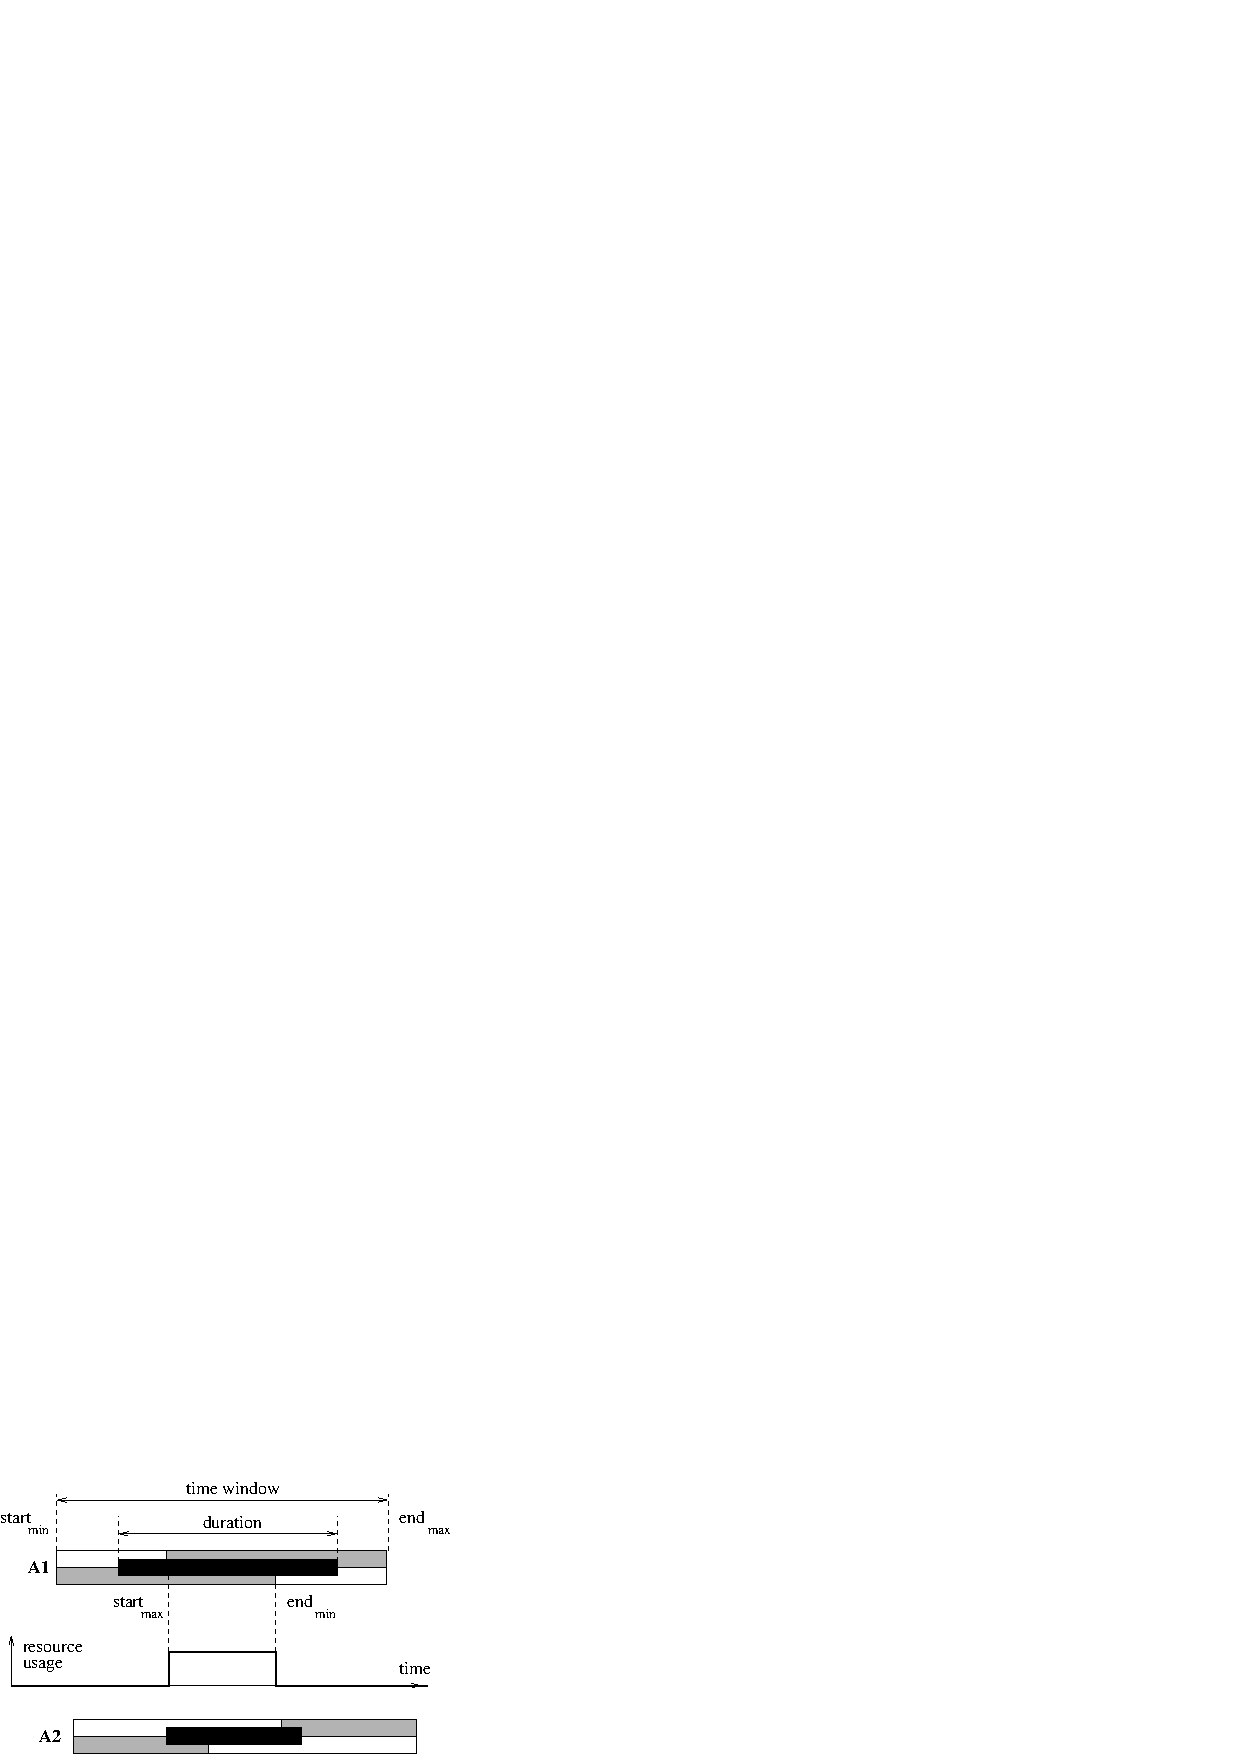
\includegraphics[width=15pc]{figures/fig1.pdf}}
\caption{Example of RTN}
\label{fig1}
\end{figure}

\begin{figure}
\centerline{\includegraphics[width=18pc]{figures/fig2.pdf}}
\caption{Solution of an RTN}
\label{fig2}
\end{figure}

\section{Expressive Power}

In this section, we show that most of the classical attributes used in
AI Planning as well as most of the resources used in Scheduling can be
represented in the RTN framework.

\subsection{Planning Attributes}

\subsubsection{STRIPS operators}
Let $p$ be a STRIPS predicate. It can be represented by a resource for
which level 0 means that $p$ is false and  level $1$ means that $p$ is
true.  Let $o$ be  an operator at time-point  $t$.   If $p$ is  in the
precondition  of operator $o$, this  can be captured by a greater-than
condition  $G(1,t',t)$ with the  constraint  $t' \prec t$\footnote{$t'
\prec t$ denotes the constraint $t-t' \in (0,+\infty)$.}.  If $\neg p$
is  in the precondition of   operator $o$, this  can  be captured by a
lower-than condition  $L(0,t',t)$.  If  $p$ is in   the delete list of
operator $o$,  this can  be captured by  an  absolute  change $A(0,t)$
stating that after $t$, $p$ will  be false. If  $p$ is in the add list
of operator $o$,  this can be captured by  an absolute change $A(1,t)$
stating that after $t$, $p$ will be true.

\subsubsection{\ixtet attributes}
Let $att$ be an \ixtet  attribute \cite{ghallab-laruelle-94}.  We  can
build a mapping $\mu_{att}$ that maps the possible values of attribute
$att$ to $\mathbb{Q}$.  Then, a  hold predicate $hold(att,v,t,t')$ can
be modeled   by an equal  condition  $E(\mu_{att}(v),t,t')$.  An event
$event(att,v,v',t)$ by   the   conjunction  of  an    equal  condition
$E(\mu_{att}(v),t',t)$, an absolute  change $A(\mu_{att}(v'),t)$ and a
temporal constraint $t' \prec t$.

\subsubsection{PDDL 2.1}
Let's consider  a durative  action of PDDL   2.1 \cite{fox-02}.   This
action can be represented  by two time points  $t_s$ (start) and $t_e$
(end) in  our formalism.   A  condition at   start on  a non-numerical
proposition   $p$  can    be captured  by    a greater-than  condition
$G(1,t,t_s)$ with the precedence $t \prec t_s$, an  effect at start by
an absolute change  $A(1,t_s)$  (similar modeling for   conditions and
effects at end) and an invariant condition by a greater-than condition
$G(1,t_s,t_e)$.  Conditions and invariants  of the form $\leq$, $\geq$
and  $=$ on numeric  variables can be captured  by RTN conditions $L$,
$G$ and $E$.  Numeric effects $assign$ correspond to absolute changes,
whereas $increase$ and $decrease$ correspond to relative changes.

\subsection{Scheduling Resources}

\subsubsection{Discrete resources}
A  discrete resource of maximal capacity  $Q$ \cite{laborie-03} can be
captured    by     an    RTN     with    a     greater-than  condition
$G(0,-\infty,+\infty)$\footnote{We assume  that   $-\infty$  denotes a
time-point before  any  other  time-point   and $+\infty$  denotes   a
time-point after any     other time-point.}  a   lower-than  condition
$L(Q,-\infty,+\infty)$ and an initial  production  $R(Q,-\infty)$.  An
activity  requiring  $q$ units of    resource over the  time  interval
$[t_s,t_e)$ is represented by  a pair of relative changes $R(-q,t_s)$,
$R(+q,t_e)$.   If the  discrete resource is   given a varying  maximal
capacity  profile,  this can   be  modeled  as   a set  of  lower-than
conditions $L(Q_i,t_i,t_{i+1})$.

\subsubsection{Reservoir}
A    reservoir  of  maximal capacity    $Q$  and  initial  level   $L$
\cite{laborie-03} can be    captured by an  RTN   with a  greater-than
condition    $G(0,-\infty,+\infty)$,      a    lower-than    condition
$L(Q,-\infty,+\infty)$  and an   absolute  change $A(L,-\infty)$.    A
production activity corresponds  to  a relative change  $R(q,t)$ where
$q>0$ whereas a consumption activity corresponds  to a relative change
$R(q,t)$ where $q<0$.

\subsubsection{State Resources}
In  ILOG Scheduler \cite{scheduler53},  state resources are defined as
objects that at each timepoint can take only  one possible state among
a known   set  of possible states   $S=\{s_i\}$.  Activities requiring
different states of the state resource cannot overlap.  We can build a
mapping $\mu_{res}$ that   maps   the possible states of    the  state
resource to $\mathbb{Q}$.  Then, the requirement of  a given state $s$
of a  state  resource by an  activity  executing on the  time interval
$[t_s,t_e)$ can be modeled as an absolute change $A(\mu_{res}(s),t_s)$
and an equal condition $E(\mu_{res}(s),t_s,t_e)$.

\subsubsection{Additional Expressivity}

The RTN framework allows for modeling complex resources and activities
in scheduling.  In  manufacturing for instance, maintenance activities
need  to be executed as  soon as the level  of some numerical variable
(measuring the ``need for  maintenance'') has reached a certain level.
The  level  of   this   variable is increased  (relative    change) by
production  activities  and  is  reset to    0 (absolute  change)   by
maintenance activities.  Another  example is scheduling while ensuring
some condition on  a numerical  variable during  the  execution of  an
activity  (e.g.   maintaining the temperature  of  a  furnace within a
suitable interval).   Such  kind of  conditions are  very important in
process industry and  chemistry.  The conjunction of absolute changes,
relative changes and  conditions holding over variable  time intervals
offers a  powerful   formalism for   representing  complex  scheduling
problems.  Additional features   such as dependence  between  variable
resource  quantities $q$ and time-points $t$  that do not directly fit
into  the  RTN model can be   handled  by additional constraints  in a
constraint propagation framework.

\section{Complexity}

In this section, we analyze  the algorithmic complexity of solving and
providing  necessary truth criteria   for general RTNs and  particular
fragments of the RTN formalism. By NP-Complete  we mean NP-Complete in
the strong sense.

\subsection{Notations}

Let us  consider the following   notations about temporal constraints:
$PA$  denotes the  point algebra    of  \cite{vilain-86} which  is   a
restriction   of STN$^{\neq}$ that   only   consists  of  the set   of
qualitative relations $\{\emptyset, \prec, \preceq, =, \succ, \succeq,
\neq, ?  \}$  between  timepoints.   $STN^{\neq}$ denotes   a  general
STN$^{\neq}$.  We write $t \prec t'$ or $t  \preceq t'$ to express the
fact  that the   corresponding relation is   subsumed  by the temporal
network.  We use   the following notations about  resource statements:
${\cal  R}^{+}$  denote any  set of   relative  changes $x$ such  that
$q(x)>0$ (producers).  ${\cal R}^{+-}_1$ denote   any set of pairs  of
resource  statements  $(R(+1,t_s),R(-1,t_e))$ where  $t_s  \prec t_e$.
${\cal     L}_Q$     denotes     the         lower-than      condition
$L(Q,-\infty,+\infty)$. ${\cal AE}$ denotes  any set of pairs  $(x,y)$
where $x=A(q,t_s)$  and $y=E(q,t_s,t_e)$   with $t_s  \prec  t_e$.   A
fragment of the complete RTN framework is denoted $(X|Y)$ where $X$ is
the set of changes and conditions allowed in this fragment and $Y$ the
type of  temporal  constraints.  $n$  denotes the  number  of resource
statements in the RTN, $m$ the  number of temporal constraints between
time-points and $\maxflow$ the complexity of  computing a maximum flow
on  a  graph  with $n$   nodes and $m$  arcs\footnote{State-of-the-art
maximum flow  algorithms   do it in     $O(nm\log n)$ in    worst case
\cite{hochbaum-98}.}.

\subsection{Finding a solution \label{solution}}
 
\begin{complexity}  
The problem of finding a solution to an RTN is in NP.
\end{complexity}

\begin{proof}
The time-consistency  of an instantiation $\sigma$   can be checked in
polynomial time and, given its definition, the function $l_\sigma$ can
be  build and the resource-consistency   checked in polynomial time. A
simple algorithm to check that an instantiation  is a solution runs in
$O(m + n \log n)$.
\end{proof}

The proof of the three polynomiality  results below is omitted because
trivial.

\begin{complexity}
$({\cal R}^{+},{\cal L}_Q|STN^{\neq})$  can be solved  in $O(n^3)$.
\end{complexity} 

%\begin{proof}
%The temporal   and resource problems   are  completely separated.  The
%temporal problem is an STN$^{\neq}$ that can be solved in $O(n^3)$. If
%temporal  constraints are consistent,  there  exists a solution to the
%RTN  if and only  if $\sum_{x \in {\cal  R}^{+}}{q(x)} \leq Q$ and, in
%this case, any time-consistent instantiation is a solution.
%\end{proof}

\begin{complexity}
$({\cal R}^{+-}_1,{\cal L}_1|PA)$ can be solved  in $O(n^3)$.
\end{complexity} 

%\begin{proof}
%This  is  a one machine  problem  submitted to precedence constraints.
%The problem can be solved by building a directed graph whose nodes are
%the pairs   of  changes in  ${\cal R}^{+-}_1$    (activities) and arcs
%represent the    existence of  a precedence   constraint  between some
%extremity of  the two activities in  the PA network.   Any topological
%sort of the directed graph is a solution to the original problem.
%\end{proof}

\begin{complexity} 
$({\cal A},{\cal R}|STN^{\neq})$ can be solved in $O(n^3)$.
\end{complexity} 

%\begin{proof}
%The problem  can be represented  as a pure  $STN^{\neq}$ by expressing
%all the original  temporal constraints and additional constraints $t_i
%\neq t_j$ if  there  exists $A(t_i,q_i)$  and $A(t_j,q_j)$  such  that
%$q_i\neq q_j$ or if there exists $A(t_i,q_i)$ and $R(t_j,q_j)$.
%\end{proof}

\begin{complexity} 
$({\cal R}^{+-}_1,{\cal L}_1|STN^{\neq})$ is NP-Complete. 
\end{complexity} 

\begin{proof}
The   scheduling decision problem $1|prec(l_{ij}),p_j=1|C_{max}\leq T$
that consists in scheduling on  a machine a  set of activities of unit
duration subject  to  min/max delays  between  activities and  maximal
makespan   is     a  special    case    of  $({\cal    R}^{+-}_1,{\cal
L}_1|STN^{\neq})$.  See for  instance \cite{finta-liu-96}  for a proof
of its NP-completeness.
\end{proof}

\begin{complexity} 
$({\cal AE}|STN^{\neq})$ is NP-Complete. 
\end{complexity} 

\begin{proof}
The special case where all the quantities $q$ of the pairs $(x,y)$ are
different  can be reformulated   as a problem $({\cal  R}^{+-}_1,{\cal
L}_1|STN^{\neq})$ (cf above).
\end{proof}

\begin{complexity} 
$({\cal R}^{+},{\cal E}|PA)$ is NP-Complete. 
\end{complexity} 

\begin{proof}
The Subset   Sum  Problem (SSP),  which is   known to   be NP-complete
\cite{garey-johnson-79} can  be reduced  to this problem.    {\em {\bf
SSP:} Given a finite set $R$; and for each element $x\in R$ a positive
integer size $q(x)$; a positive integer $Q$.  Is there a subset $S$ of
$R$ such that $\sum_{x \in S}{q(x)} = Q$?  }   Let the RTN composed of
the resource relative  changes $R(q(x),t(x))$ for $x  \in R$  and only
one  equal condition $E(Q,\tau,\tau')$  with $\tau \prec \tau'$.  It's
clear  that  if there exists  a solution   $S$  to the  SSP  then this
solution can  clearly be transformed into a  solution  to the RTN; for
example by  choosing $\tau=0$, $\tau'=1$, $\forall   x \in S, t(x)=0$,
$\forall x \in R \setminus S, t(x)=1$.  Reciprocally, for any solution
$\sigma$ to the RTN, a solution to the corresponding  SSP can be built
by    taking    $S=\{x     \in   R   /   \sigma\!\circ\!t(x))     \leq
\sigma(\tau)\}$. Note that SSP is not NP-Complete in the strong sense.
$({\cal  R}^{+},{\cal E}|PA)$ can be  proved to be  NP-Complete in the
strong  sense   by a   transformation   from the  3-Partition  problem
\cite{garey-johnson-79}  very     similar  to the   one   used in this
proof.
\end{proof}

\begin{complexity} 
$({\cal A},{\cal R}^{+},{\cal L}_Q|PA)$ is NP-Complete. 
\end{complexity} 

\begin{proof}
The Bin Packing   Problem (BPP),  which   is known to be   NP-complete
\cite{garey-johnson-79} can  be  reduced to this problem.    {\em {\bf
BPP:} Given a finite set  $R$ of $m$ items; for  each item $x \in R$ a
positive  integer size $q(x)$; a positive  integer $Q$ and $k \leq m$.
Can $R$ be partitioned into $k$  disjoint sets $R_1,...,R_k$ such that
$\forall  i \in [1,k],  \sum_{x  \in R_i}{q(x)}\leq  Q$?}  Let the RTN
composed of the  resource  relative changes  $\{R(q(x),t(x))\}_{x  \in
{\cal     R}}$,    a temporal   chain     of   $k-1$ absolute  changes
$\{A(0,\tau_i)\}_{i=1..k-1}$ with  the precedence constraint   $\tau_i
\prec \tau_{i+1}$ and the lower-than condition $L(Q,-\infty,+\infty)$.
If there exists a solution $R_1,...,R_k$ to the BPP, it's clear that a
solution $\sigma$ to the RTN can be  built as follows: $\sigma(\tau_i)
= 2i$, $\forall x \in R_i, \sigma\!\circ\!t(x)=2i-1$.  Reciprocally, a
solution to the RTN problem can be used to build a solution to the BPP
by defining the sets $R_1 = \{ x \in {\cal R} / \sigma\!\circ\!t(x) <
\sigma(\tau_1) \}$ and, for $1<i<k$, $R_i = \{ x \in {\cal R} /
\sigma(\tau_{i-1}) \leq  \sigma\!\circ\!t(x) < \sigma(\tau_{i})\}$ and
$R_k = \{ x \in {\cal R} / \sigma(\tau_{k-1}) \leq \sigma\!\circ\!t(x)
\}$.
\end{proof}

\begin{complexity} 
$({\cal R}^{+-}_1,{\cal L}_Q|PA)$ is NP-Complete. 
\end{complexity} 

\begin{proof}
The Sequencing to   Minimize Maximum Cumulative Cost  Problem (SMMCCP)
with tasks costs  in  $\{-1,1\}$, which  is  known to  be  NP-complete
\cite{garey-johnson-79}  can be  reduced to  this  problem. {\em  {\bf
SMMCCP:}  Given a set  of tasks  $T$,   a partial order  between tasks
$\prec$, a fixed cost $c(t) \in \{-1,1\}$ for each  task $t \in T$ and
a constant $K$, find a  total order $<$  on $T$ that obeys the partial
order $\prec$ and such that $\forall t \in T, \sum_{t' < t} c(t') \leq
K$.} Given a SMMCCP,   we can build an  RTN as follows.  Each task $t$
corresponds to  a time-point in the   RTN.  The precedence constraints
correspond  to the partial order $\prec$ between tasks. Two additional
time-points $-\infty$ and $+\infty$ are  respectively added before and
after all the other time points $t \in  T$.  For a  task $t$ such that
$c(t)=+1$, we  add      the  two relative   changes    $R(+1,t)$   and
$R(-1,+\infty)$. For a  task $t$ such  that $c(t)=-1$, we add  the two
relative changes $R(+1,-\infty)$ and $R(-1,t)$.  Let $N$ be the number
of tasks $t$ such that $c(t)=-1$. We then add the lower-than condition
$L(K+N, -\infty, +\infty)$.  Let  $i(t)  \in [1,|T|]$ be an  arbitrary
indexing of the  set of tasks $T$.  Let  $\sigma$ be a solution to the
RTN.  We build a total order  between tasks as  follows: $t'<t$ if and
only  if   $\sigma(t')<\sigma(t)$    or  [$\sigma(t')=\sigma(t)$   and
$c(t')=-1$ and $c(t)=+1$]  or [$\sigma(t')=\sigma(t)$ and $c(t')=c(t)$
and $i(t')<i(t)$].   It's easy to see  that $<$ is   a solution to the
original SMMCCP.
\end{proof}
 
\subsection{Necessary Truth Criterion}

The Necessary Truth Criterion (NTC) is the problem of deciding whether
a given  RTN is such that  any of its time-consistent instantiation is
also resource-consistent    (and thus,  is a   solution).    NTCs were
introduced   by David   Chapman    in    a very   influential    paper
\cite{chapman-87} where, in the context of planning with resources, he
mentions the  existence  of {\em ``clever  polynomial algorithms using
network flow techniques that  compute the exact  least value the state
variable could take on''}.   One  of these algorithms was described in
\cite{rhys-70} and  more  recently in \cite{muscettola-02}.    In this
section, we develop  this idea  and  give some complexity results  for
NTCs in the context of resource temporal networks. Notice that, due to
lack of   space, proofs are mostly  sketched.  Note also that  all the
problems    studied in  this   section  are   NP-Complete (see section
\ref{solution}).  Without lack of generality we assume in this section
that the RTNs  do  not contain  any  potentially conflicting pairs  of
changes. A pair of absolute changes $(x,x') \in {\cal A}^2$ is said to
be potentially conflicting if and only if $q(x) \neq q(x')$ and ${\cal
N}$ does  not  subsume $t(x) \neq   t(x')$.  A pair $(x,x')  \in {\cal
A}\times {\cal R}$ is  said to be  potentially conflicting if and only
if  ${\cal N}$ does  not subsume  $t(x) \neq t(x')$.  Indeed, if  such
conflicting  pairs    exist, it  is  easy    to add  the corresponding
non-simultaneity  constraints $t(x)   \neq   t(x')$  on ${\cal N}$.

\begin{lemma} 
\label{lemma1}
NTC  for  $({\cal   R},{\cal   L}_Q|STN^{\neq})$ can   be   solved  in
$O(\maxflow)$.
\end{lemma} 

\begin{proof}
First, we  recap   a result of  \cite{rhys-70}   showing that  NTC for
$({\cal  R},{\cal  L}_Q|PA  )$  is  polynomial.  The  problem   can be
expressed as  a Maximum Weight Closure Problem  (MWCP) on the directed
graph  where the arcs  $\prec$, $\preceq$ of  the PA network have been
reversed and  all arcs $\neq$ are ignored.   {\em {\bf  MWCP:} Given a
directed graph $G=(V,A)$  and a node  weight $q(x) \in \mathbb{Q}$ for
each node in $x \in V$.  A subset $S  \subseteq V$ is called a closure
if and only if it does not contain any outgoing arc that is $\forall x
\in S, (x,y) \in A \Rightarrow  y \in S$.  The problem  is to find the
maximum weight closure.}  The RTN satisfies the NTC if and only if the
weight of  the  maximum  weight closure   is lower than   or equal  to
$Q$. Indeed, if $S^*$ denotes the maximum weight closure, there exists
an instantiation of  the RTN such  that all the  changes in $S^*$  are
scheduled  before all the other  changes and the  resource level after
all the changes in  $S^*$ is the  maximum resource level reachable  in
all time-consistent instantiations.  This level  is exactly the weight
of $S^*$.  As shown in  \cite{ahuja-book}, the  MWCP is equivalent  to
the min-cut/max-flow  problem.   For the more general  problem $({\cal
R},{\cal      L}_Q|STN^{\neq})$,     similar   arguments      as    in
\cite{muscettola-02} ({\em  separation schedule}) can  be used to show
that the  RTN satisfies the  NTC if and  only  if the  symbolical $PA$
temporal constraint network subsumed by the $STN^{\neq}$ satisfies the
NTC.
\end{proof}

\begin{lemma} 
\label{lemma2}
NTC  for $({\cal A},{\cal R^{+}},{\cal   L}_Q|PA)$  can be solved   in
$O(\maxflow)$.
\end{lemma} 
 
\begin{proof}
We  can  note  that   for  any  instantiation  $\sigma$,   the set  of
chronologically ordered  absolute changes  ${\cal A}=\{x_i\}_{i=1..n}$
with $\sigma \circ t(x_i) \leq \sigma \circ t(x_{i+1})$ partitions the
set of changes ${\cal A} \cup {\cal R^{+}}$ into $n+1$ subsets: $S_0 =
\{ y \in {\cal R^{+}}, \sigma \circ t(y) < \sigma \circ t(x_1)\}$, for
$i=1..n-1$, $S_i = \{ x_i \} \cup \{ y  \in {\cal R^{+}}, \sigma \circ
t(x_i) < \sigma \circ  t(y) <  \sigma  \circ t(x_{i+1})\}$, $S_n  = \{
x_n\} \cup \{ y  \in {\cal R^{+}}, \sigma  \circ t(x_n) < \sigma \circ
t(y)\}$.  $S_i$  is called the layer of  $x_i$.  In  this context, the
maximal level of the resource  in instantiation $\sigma$ is the weight
of  the maximum weight  layer $S\subseteq {\cal  A} \cup {\cal R^{+}}$
defined as $\sum_{x \in S}{q(x)}$.  Given an instance of RTN, we build
an undirected graph $G$ as follows.  Each change  $x \in {\cal A} \cup
{\cal R^{+}}$ is associated a unique node in $G$ whose weight is equal
to $q(x)$.   Informally, there will  be  an  edge between two  changes
$\{x,x'\}$  if and only if they  cannot belong to  the same layer in a
time-consistent instantiation.   More precisely,  there is an  edge in
$G$ between each pair of absolute change. Furthermore, if $x \in {\cal
A} \cup {\cal  R^{+}}$  is a  change  and $x'  \in {\cal R^{+}}$  is a
relative change, there is  an edge  $\{x,x'\}$ in $G$  if and  only if
there exists an absolute change $y \in  {\cal A}$ such that $x \preceq
y \preceq x'$.  It is not difficult to show that  the maximal level of
the resource is equal to the weight  of the maximum independent set of
$G$.  Furthermore $G$ is a comparability graph  as the edges involving
at   least one  relative change   can naturally  be oriented with  the
direction of a path containing an absolute change between them and the
remaining  of the  edges (between  pairs of  absolute changes) forms a
clique.     Computing  the   maximum  weight  independent    set  of a
comparability  graph  is polynomial  and can be  solved  as a min-flow
problem \cite{golumbic-80}.   Thus, the NTC  only needs to compare the
weight of  the maximum weight independent  set of $G$ with the maximal
resource level $Q$.
\end{proof}

The following lemma is a generalization of Lemma \ref{lemma2} when all
changes are allowed including consumers ($q<0$).

\begin{lemma} 
\label{lemma3}
NTC  for $({\cal A},{\cal    R},{\cal   L}_Q|PA)$ can be  solved    in
$O(n\,\maxflow)$.
\end{lemma} 

\begin{proof}
We prove   that the problem  can  be solved  by solving  $n_A$ Maximum
Weight Convex Set Problems (MWCSP) where $n_A \leq n$ is the number of
absolute changes.  {\em {\bf MWCSP:} Given  a poset $G=(V,\leq$) where
$\leq$  is  a partial  order   on $V$  (reflexive,  antisymmetric  and
transitive relation)  and a weight  function  $w(x)\in \mathbb{Q}$.  A
subset $S \subseteq V$  is said to be convex  if and only  if $\forall
(x,y) \in S^2, \forall z \in V, x \leq z  \leq y \Rightarrow z \in S$.
The problem  is  to find a  convex  subset $S \subseteq  V$ of maximum
total  weight.} As  shown  in \cite{groflin-85},  this  problem can be
solved in polynomial   time by a  min-flow/max-cut  algorithm.   For a
given absolute change $x_i \in {\cal A}$, we  transform the problem of
computing the maximum level of the resource in the layer of $x_i$ (see
sketch of proof of  Lemma \ref{lemma2}) as an  instance of MWCSP.  The
poset $G_i=(V_i,\leq)$ of this MWCSP is built as follows: $V_i=\{x_i\}
\cup \{x \in {\cal A}  \cup {\cal R},  \neg(x \preceq x_i)\}$  and  $x
\leq y$  if and only if relation  $x \preceq y$  is subsumed by the PA
network. $w(x_i)=K+q(x_i)$ where $K$ is  big enough ($K >\Sigma_{x \in
{\cal R}}{|q(x)|}$),  $w(x)=-\infty$  if  $x  \in  {\cal A}  \setminus
\{x_i\}$ and  $w(x)=q(x)$ if $x \in {\cal  R}$.  One can show that for
any  convex set  $S$  of  $G_i$  containing   $x_i$, there   exists  a
time-consistent  instantiation $\sigma$ and   a   time $t$ such   that
$l_\sigma(t)=w(S)-K$ and  that  for any  time-consistent instantiation
$\sigma$ and  a time $t$,  the  set $\{ x \in V_i / \sigma \circ  t(x)
\leq t \}$  is convex.  Thus,  the maximum resource level reachable in
the layer of $x_i$ is $w(S_i^*)-K$ where $S_i^*$ is the maximum weight
convex set of  $G_i$.  Note that due to   the choice of $K$, $x_i  \in
S_i^*$.
\end{proof}

We  can  see that Lemmas   \ref{lemma1}, \ref{lemma2} and \ref{lemma3}
also hold when the unique lower-than condition does  not span over the
complete   horizon   $(-\infty,+\infty)$  but  on  some  variable time
interval $[t_s,t_e)$ where  $\{t_s,t_e\}\subset {\cal T}$.  Indeed, in
this case,  the problem  can be transformed  into a  problem where the
lower-than   condition  spans  over the   complete  horizon  and three
additional  relative  changes   are     considered:   $R(-K,-\infty)$,
$R(+K,t_s)$, $R(-K,t_e)$ where $K$ is big enough.

Furthermore, Lemmas \ref{lemma1}   and  \ref{lemma3} also  hold  for a
greater-than  condition ${\cal G}_Q$ as,   here again, the problem can
easily be transformed into   a  problem with a lower-than    condition
${\cal L}_{-Q}$ and with opposite resource changes. 

\begin{theorem}
\label{decomposability}
Let ${\Pi}=({\cal T},{\cal A},{\cal R},{\cal L},{\cal G},{\cal N})$ be
an RTN. For $y \in {\cal L} \cup {\cal G}$, let $\Pi_y$ denote the RTN
where y is the only condition in  other words $\Pi_y = ({\cal T},{\cal
A},{\cal  R},{\cal   L}\cap    \{y\},{\cal G}\cap   \{y\},{\cal  N})$.
$NTC({\Pi})$ is true if  and only if  for each condition statement  $y
\in {\cal L} \cup {\cal G}$, $NTC({\Pi_y})$ is true.
\end{theorem}

\begin{proof}
The theorem  gives a necessary  condition for $NTC({\Pi})$  to be true
because if  the condition is  not met, a time-consistent instantiation
can be    built that is   not resource-consistent.    Reciprocally, if
$NTC({\Pi})$  is false, it  means that there  exists a time-consistent
instantiation that  is not  resource-consistent.  This time-consistent
instantiation violates at least one condition statement $y\in {\cal L}
\cup {\cal G}$.
\end{proof}

The following  complexity results use Theorem \ref{decomposability} to
extend Lemmas \ref{lemma1} and  \ref{lemma3} to the more general  case
of any set of  condition statements.  For  each of these  results, one
can  show that problem  $\Pi_y$ can  be  transformed  into one  of the
corresponding lemma and thus, its time complexity is polynomial.

\begin{complexity}
NTC  for $({\cal R},{\cal  L},{\cal  G}|STN^{\neq})$ can  be solved in
$O(n\,\maxflow)$.
\end{complexity} 

\begin{complexity}
NTC  for $({\cal A},{\cal R},{\cal L},{\cal  G}|PA)$  can be solved in
$O(n^2\,\maxflow)$.
\end{complexity} 

\section{Conclusion and Future Work}

In this paper, we introduce the notion of RTN to express a large panel
of possible evolutions of a  given numerical state variable over time.
RTNs  allow  modeling on  the   same fluent features of   classical AI
Planning  (absolute  changes,  conditions)  and   Scheduling (relative
changes). We show that  computing a solution to  an RTN is in  general
NP-Complete   whereas    determining    whether   all  time-consistent
instantiations of an RTN are solutions is polynomial. This last result
indicates that efficient    solving methods based  on such  polynomial
Necessary Truth Criteria  can be developed.  Indeed,  when an RTN does
not satisfy  the NTC,  all the   algorithms we  mention can exhibit  a
subset  of changes  sufficient  to  explain why  some  time-consistent
instantiations are not a solution.  Just like in classical planning or
scheduling,  these potential  conflicts can  be  used  to  branch in a
search tree  until   the NTC    is true   and  to perform   constraint
propagation.

A direction for future work will consist in studying the complexity of
the only problem  whose  complexity is  still  open: NTC  for  $({\cal
A},{\cal  R},{\cal  L},{\cal  G}|STN^{\neq})$.   Based on   the fairly
optimistic results described  in this paper, we also  plan to  work on
the development of practical and efficient  algorithms for solving NTC
and for  finding solutions (branching schemes, heuristics, computation
of resource envelopes,  constraint  propagation).  We think   that the
numerous   and well-studied  combinatorial  problems  we found tightly
related with RTNs  (one-machine scheduling  problems, subset sum,  bin
packing, sequencing to   minimize  maximum cumulative  costs,  maximum
weight closure, maximum weight  independent set, maximum weight convex
set) can also help to solve  RTNs.  For instance, state-of-the-art bin
packing   algorithms could be   a  source of   inspiration for $({\cal
A},{\cal R}^+,{\cal L}_Q|STN^{\neq})$.   Extension of the framework to
integrate   and mix    continuous  relative changes   (see  continuous
reservoirs     \cite{scheduler53}) and     absolute      changes  (see
\cite{penberthy-weld-94,trinquart-ghallab-01})   is  also clearly   of
interest.

\section{Acknowledgements}

I am very  grateful to Andr\'e Kezdy for  pointing me to some relevant
articles about the maximum weight  convex  set problem  as well as  to
many  other  graph theorists  who  got   interested in  this  problem.
Special  thanks  to   Emmanuel   Gu\'er\'e and Pascal   Massimino  for
enlightening  discussions on the  RTN semantics  and complexity issues
and to Francis Sourd for carefully proofreading the paper.

\bibliographystyle{named}
\bibliography{ilog-03-002}
\end{document}
